\documentclass{article}\usepackage[]{graphicx}\usepackage[]{color}
%% maxwidth is the original width if it is less than linewidth
%% otherwise use linewidth (to make sure the graphics do not exceed the margin)
\makeatletter
\def\maxwidth{ %
  \ifdim\Gin@nat@width>\linewidth
    \linewidth
  \else
    \Gin@nat@width
  \fi
}
\makeatother

\definecolor{fgcolor}{rgb}{0.345, 0.345, 0.345}
\newcommand{\hlnum}[1]{\textcolor[rgb]{0.686,0.059,0.569}{#1}}%
\newcommand{\hlstr}[1]{\textcolor[rgb]{0.192,0.494,0.8}{#1}}%
\newcommand{\hlcom}[1]{\textcolor[rgb]{0.678,0.584,0.686}{\textit{#1}}}%
\newcommand{\hlopt}[1]{\textcolor[rgb]{0,0,0}{#1}}%
\newcommand{\hlstd}[1]{\textcolor[rgb]{0.345,0.345,0.345}{#1}}%
\newcommand{\hlkwa}[1]{\textcolor[rgb]{0.161,0.373,0.58}{\textbf{#1}}}%
\newcommand{\hlkwb}[1]{\textcolor[rgb]{0.69,0.353,0.396}{#1}}%
\newcommand{\hlkwc}[1]{\textcolor[rgb]{0.333,0.667,0.333}{#1}}%
\newcommand{\hlkwd}[1]{\textcolor[rgb]{0.737,0.353,0.396}{\textbf{#1}}}%
\let\hlipl\hlkwb

\usepackage{framed}
\makeatletter
\newenvironment{kframe}{%
 \def\at@end@of@kframe{}%
 \ifinner\ifhmode%
  \def\at@end@of@kframe{\end{minipage}}%
  \begin{minipage}{\columnwidth}%
 \fi\fi%
 \def\FrameCommand##1{\hskip\@totalleftmargin \hskip-\fboxsep
 \colorbox{shadecolor}{##1}\hskip-\fboxsep
     % There is no \\@totalrightmargin, so:
     \hskip-\linewidth \hskip-\@totalleftmargin \hskip\columnwidth}%
 \MakeFramed {\advance\hsize-\width
   \@totalleftmargin\z@ \linewidth\hsize
   \@setminipage}}%
 {\par\unskip\endMakeFramed%
 \at@end@of@kframe}
\makeatother

\definecolor{shadecolor}{rgb}{.97, .97, .97}
\definecolor{messagecolor}{rgb}{0, 0, 0}
\definecolor{warningcolor}{rgb}{1, 0, 1}
\definecolor{errorcolor}{rgb}{1, 0, 0}
\newenvironment{knitrout}{}{} % an empty environment to be redefined in TeX

\usepackage{alltt}

\usepackage[utf8]{inputenc}
\usepackage{hyperref}
\usepackage{booktabs}
\usepackage{longtable}
\usepackage{array}
\usepackage{multirow}
\usepackage[table]{xcolor}
\usepackage{wrapfig}
\usepackage{float}
\usepackage{colortbl}
\usepackage{pdflscape}
\usepackage{tabu}
\usepackage{threeparttable}
\usepackage{threeparttablex}
\usepackage[normalem]{ulem}
\usepackage{makecell}

\hypersetup{
    linktocpage,
    colorlinks=true, 
    linkcolor=blue,
    citecolor=blue,
    filecolor=blue,
    urlcolor=blue
}
\IfFileExists{upquote.sty}{\usepackage{upquote}}{}
\begin{document}

\title{AP2G Chip-Seq Comparisons}
\author{Lucas Michel Todó}
\maketitle
\tableofcontents
\clearpage





\section{Taules Resum}
\subsection{Regió 5'}
\begin{knitrout}
\definecolor{shadecolor}{rgb}{0.969, 0.969, 0.969}\color{fgcolor}\begin{table}[H]
\centering\rowcolors{2}{gray!6}{white}

\begin{tabular}{lrrrr}
\hiderowcolors
\toprule
  & 3D7 & B11 & E5HA & NF54\\
\midrule
\showrowcolors
Min. & 0.0 & 1.6 & 0.4 & 0.2\\
1st Qu. & 4.6 & 20.5 & 6.1 & 6.4\\
Median & 17.2 & 46.9 & 24.8 & 17.8\\
Mean & 23.4 & 45.1 & 31.2 & 21.5\\
3rd Qu. & 38.6 & 67.7 & 53.6 & 35.5\\
Max. & 103.4 & 122.8 & 126.1 & 79.7\\
\bottomrule
\end{tabular}
\rowcolors{2}{white}{white}
\end{table}


\end{knitrout}
\subsection{ORF}
\begin{knitrout}
\definecolor{shadecolor}{rgb}{0.969, 0.969, 0.969}\color{fgcolor}\begin{table}[H]
\centering\rowcolors{2}{gray!6}{white}

\begin{tabular}{lrrrr}
\hiderowcolors
\toprule
  & 3D7 & B11 & E5HA & NF54\\
\midrule
\showrowcolors
Min. & 9.9 & 29.5 & 22.4 & 13.2\\
1st Qu. & 70.8 & 109.6 & 94.4 & 73.5\\
Median & 92.8 & 129.9 & 118.8 & 87.4\\
Mean & 88.8 & 128.8 & 114.9 & 91.2\\
3rd Qu. & 107.3 & 149.1 & 138.6 & 103.4\\
Max. & 161.7 & 216.0 & 211.0 & 202.9\\
\bottomrule
\end{tabular}
\rowcolors{2}{white}{white}
\end{table}


\end{knitrout}
\subsection{Regió 3'}
\begin{knitrout}
\definecolor{shadecolor}{rgb}{0.969, 0.969, 0.969}\color{fgcolor}\begin{table}[H]
\centering\rowcolors{2}{gray!6}{white}

\begin{tabular}{lrrrr}
\hiderowcolors
\toprule
  & 3D7 & B11 & E5HA & NF54\\
\midrule
\showrowcolors
Min. & 0.7 & 4.7 & 1.7 & 4.1\\
1st Qu. & 2.9 & 9.1 & 4.4 & 7.6\\
Median & 5.1 & 22.5 & 5.7 & 11.9\\
Mean & 5.7 & 23.5 & 6.7 & 13.4\\
3rd Qu. & 7.3 & 34.0 & 8.6 & 17.3\\
Max. & 19.5 & 76.9 & 22.5 & 48.4\\
\bottomrule
\end{tabular}
\rowcolors{2}{white}{white}
\end{table}


\end{knitrout}
\clearpage




\section{Gràfics}
\subsection{Coverage}
\begin{knitrout}
\definecolor{shadecolor}{rgb}{0.969, 0.969, 0.969}\color{fgcolor}
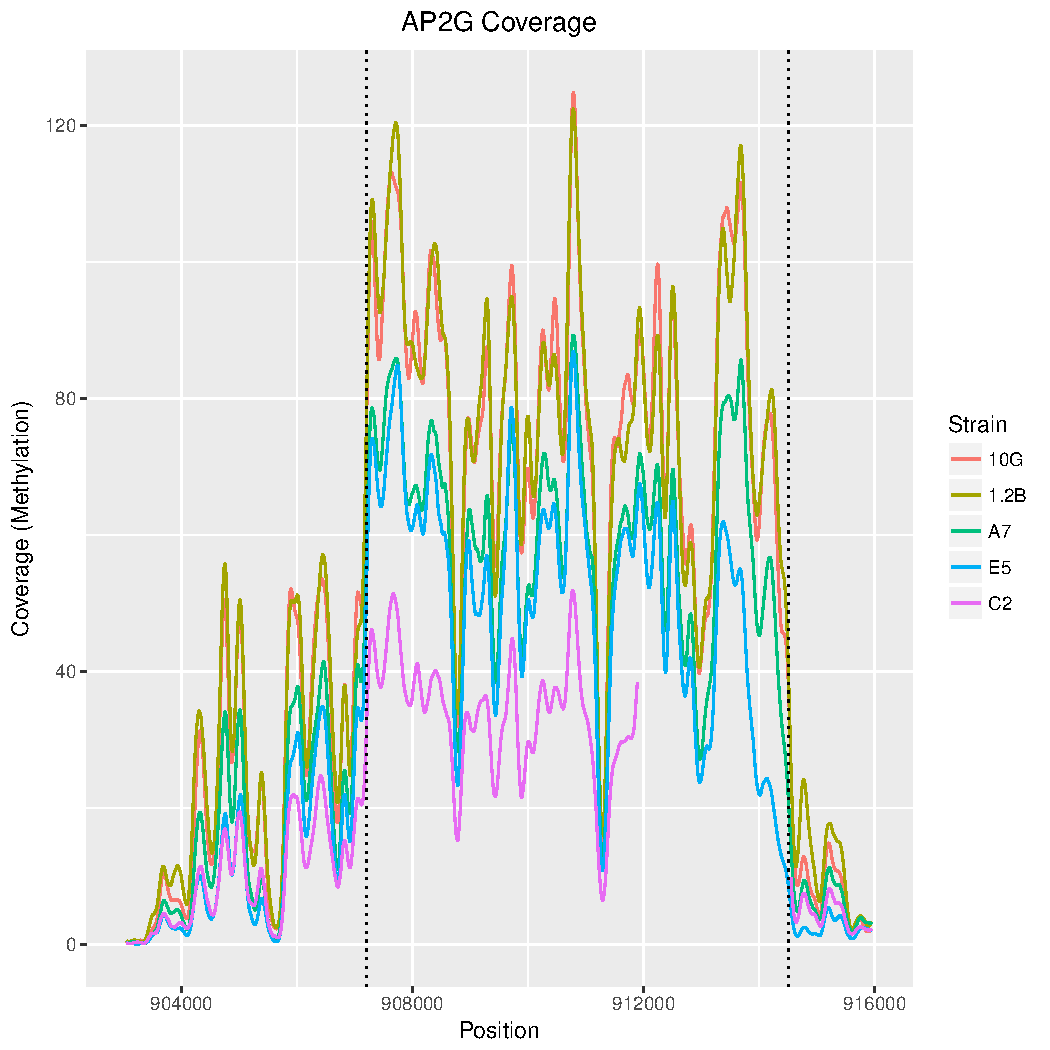
\includegraphics[width=1\linewidth]{figure/plot_coverage-1} 

\end{knitrout}
\clearpage
\subsection{Coverage Normalitzat}
\begin{knitrout}
\definecolor{shadecolor}{rgb}{0.969, 0.969, 0.969}\color{fgcolor}
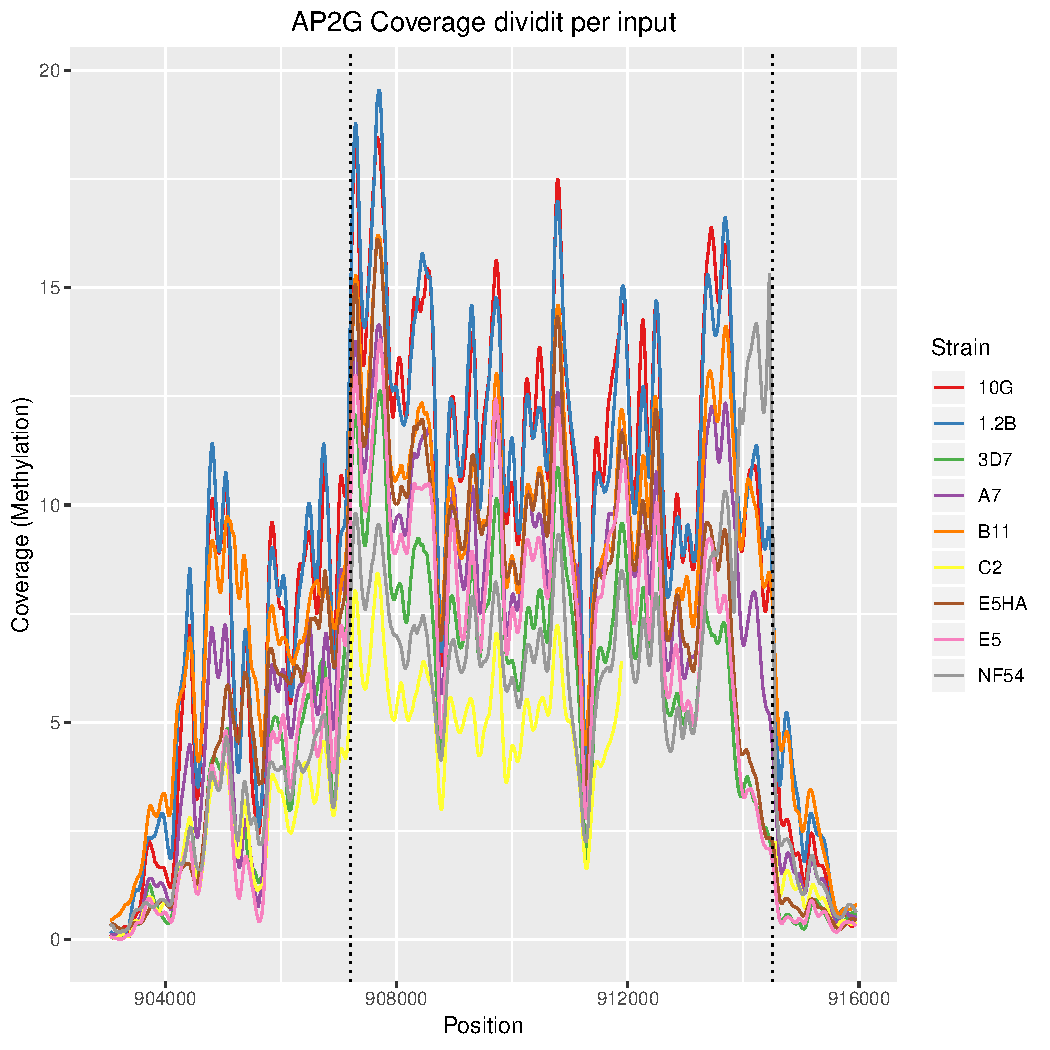
\includegraphics[width=1\linewidth]{figure/plot_norm_cov-1} 

\end{knitrout}
\clearpage
\subsection{Coverage "Equalitzat"}
\begin{knitrout}
\definecolor{shadecolor}{rgb}{0.969, 0.969, 0.969}\color{fgcolor}
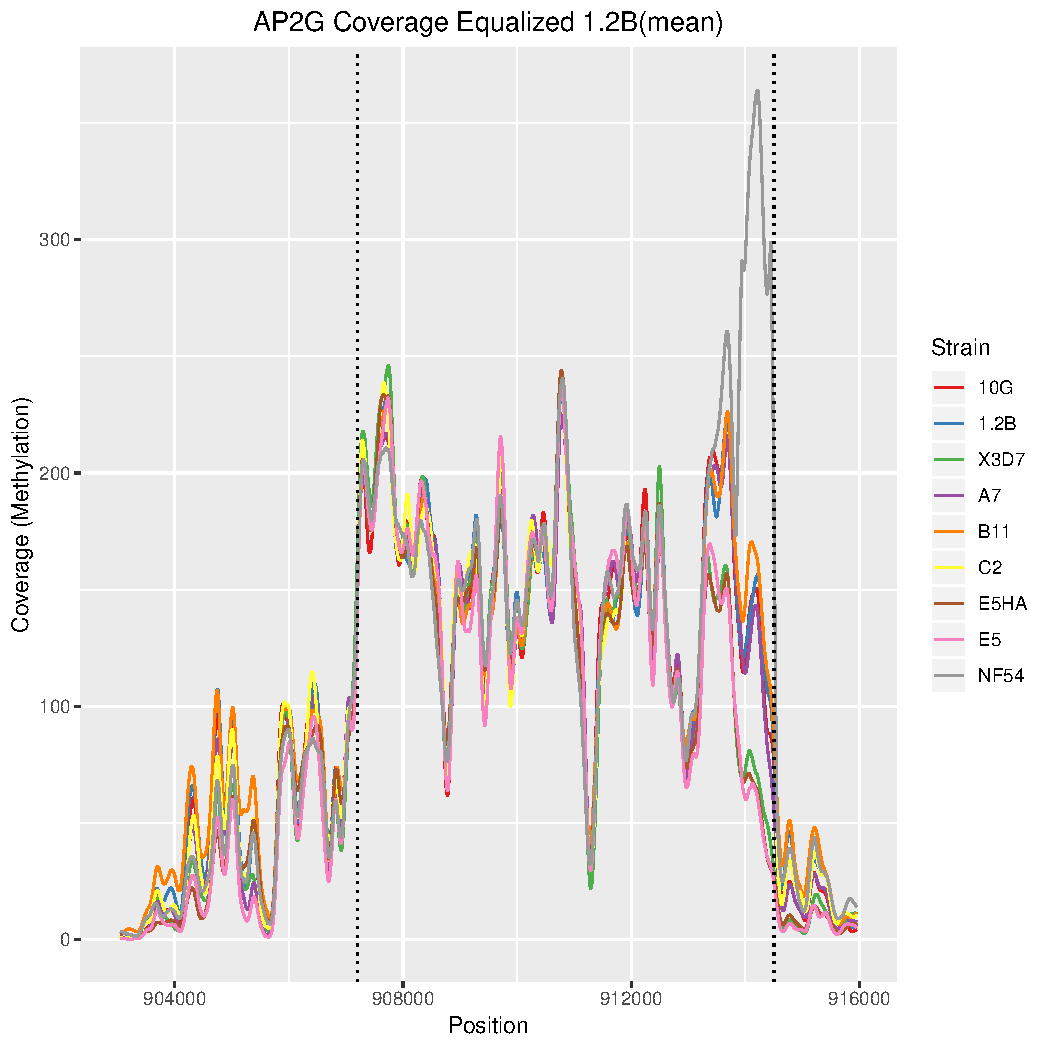
\includegraphics[width=1\linewidth]{figure/plot_equalizedCov-1} 

\end{knitrout}
\clearpage
\subsection{Coverage Normalitzat i "Equalitzat"}
\begin{knitrout}
\definecolor{shadecolor}{rgb}{0.969, 0.969, 0.969}\color{fgcolor}
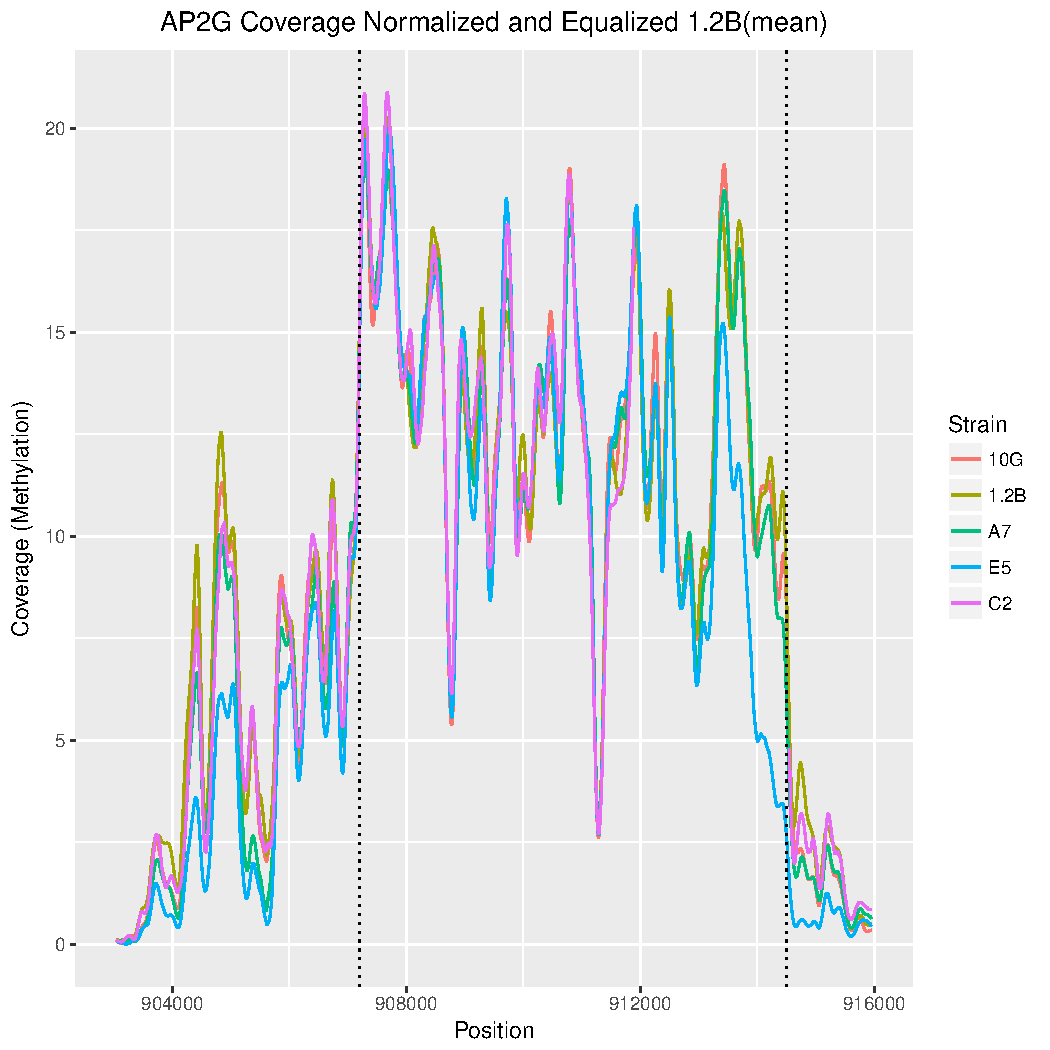
\includegraphics[width=1\linewidth]{figure/plot_NormequalizedCov-1} 

\end{knitrout}
\clearpage
\subsection{Coverage Normalitzat a regió 5'}
\begin{knitrout}
\definecolor{shadecolor}{rgb}{0.969, 0.969, 0.969}\color{fgcolor}
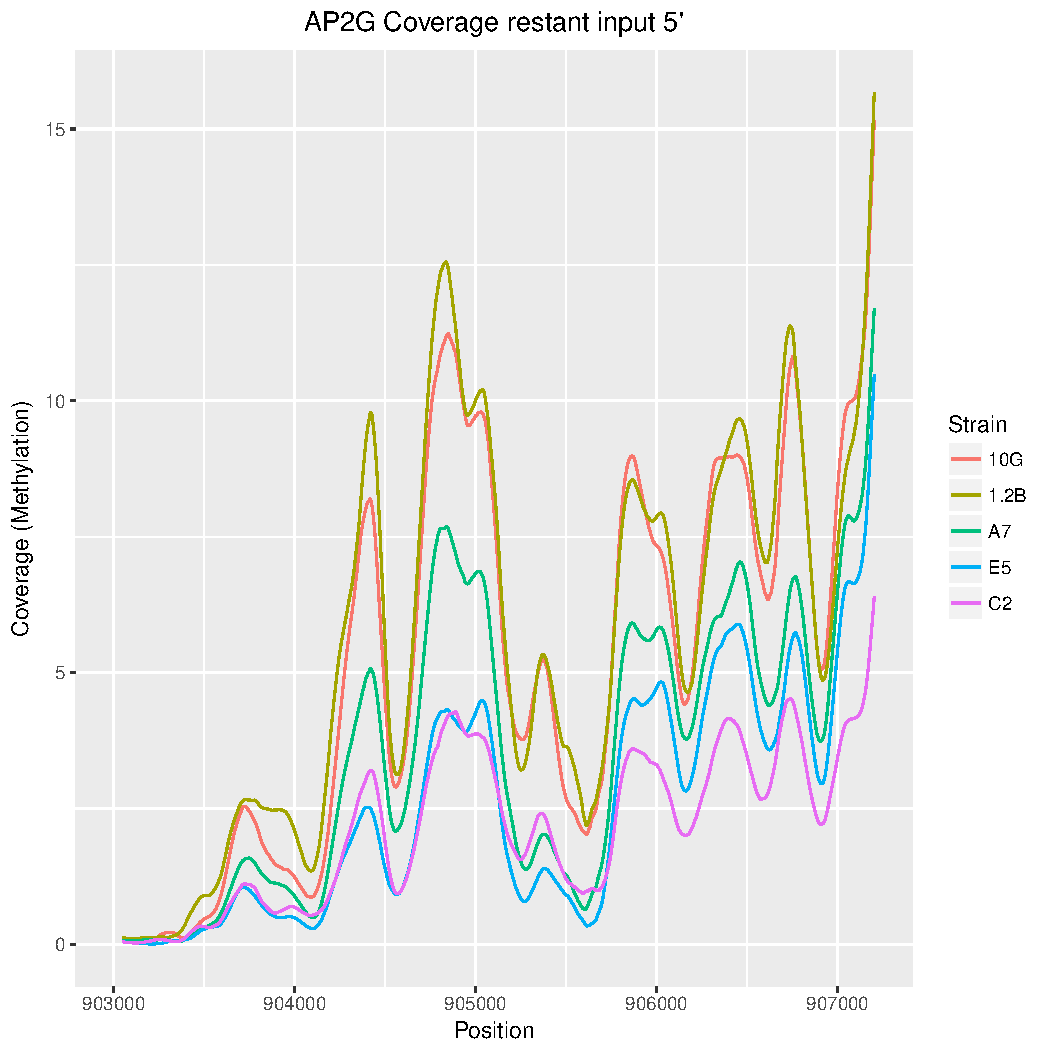
\includegraphics[width=1\linewidth]{figure/plot_norm_cov_5-1} 

\end{knitrout}
\clearpage
\subsection{Coverage Acetilació}
\begin{knitrout}
\definecolor{shadecolor}{rgb}{0.969, 0.969, 0.969}\color{fgcolor}
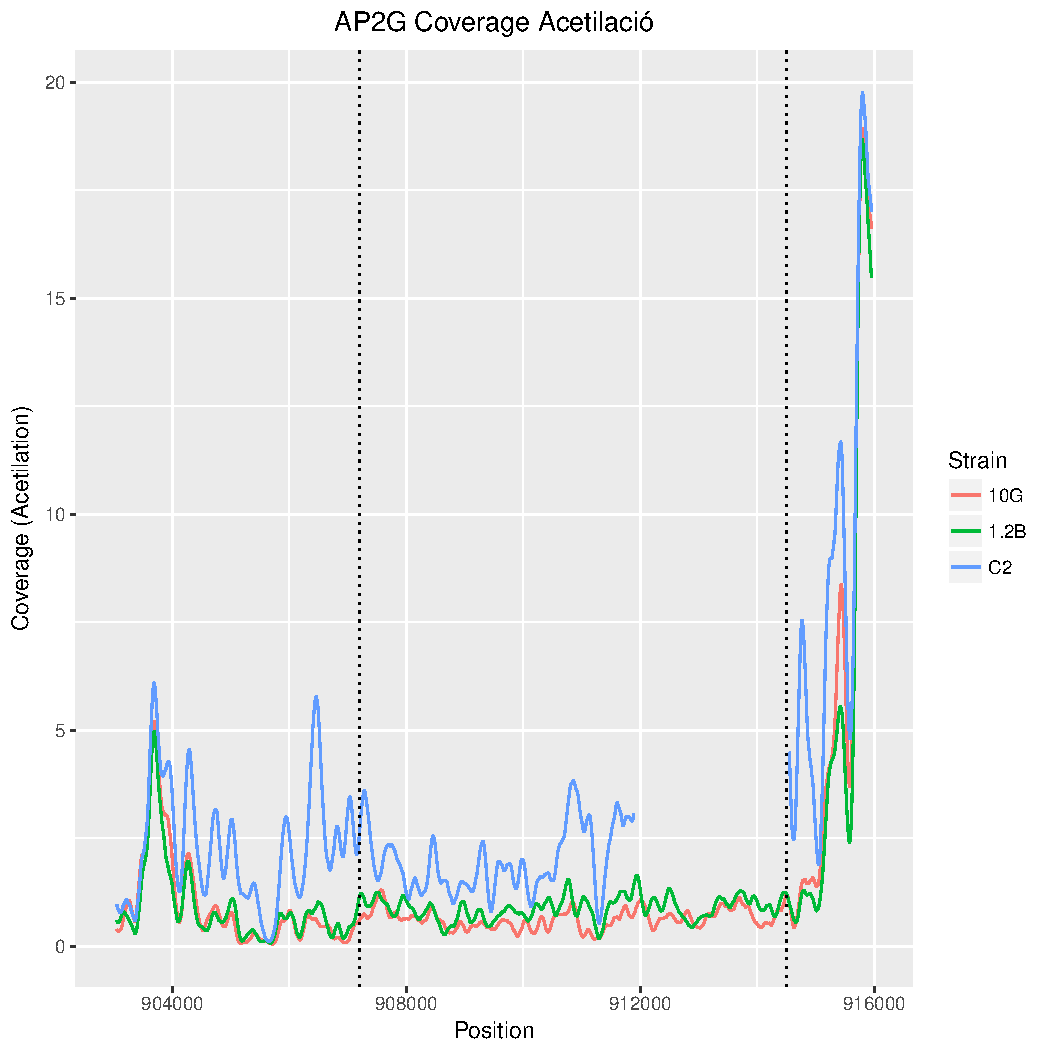
\includegraphics[width=1\linewidth]{figure/plot_ac-1} 

\end{knitrout}
\clearpage
\subsection{Coverage Acetilació a 5'}
\begin{knitrout}
\definecolor{shadecolor}{rgb}{0.969, 0.969, 0.969}\color{fgcolor}
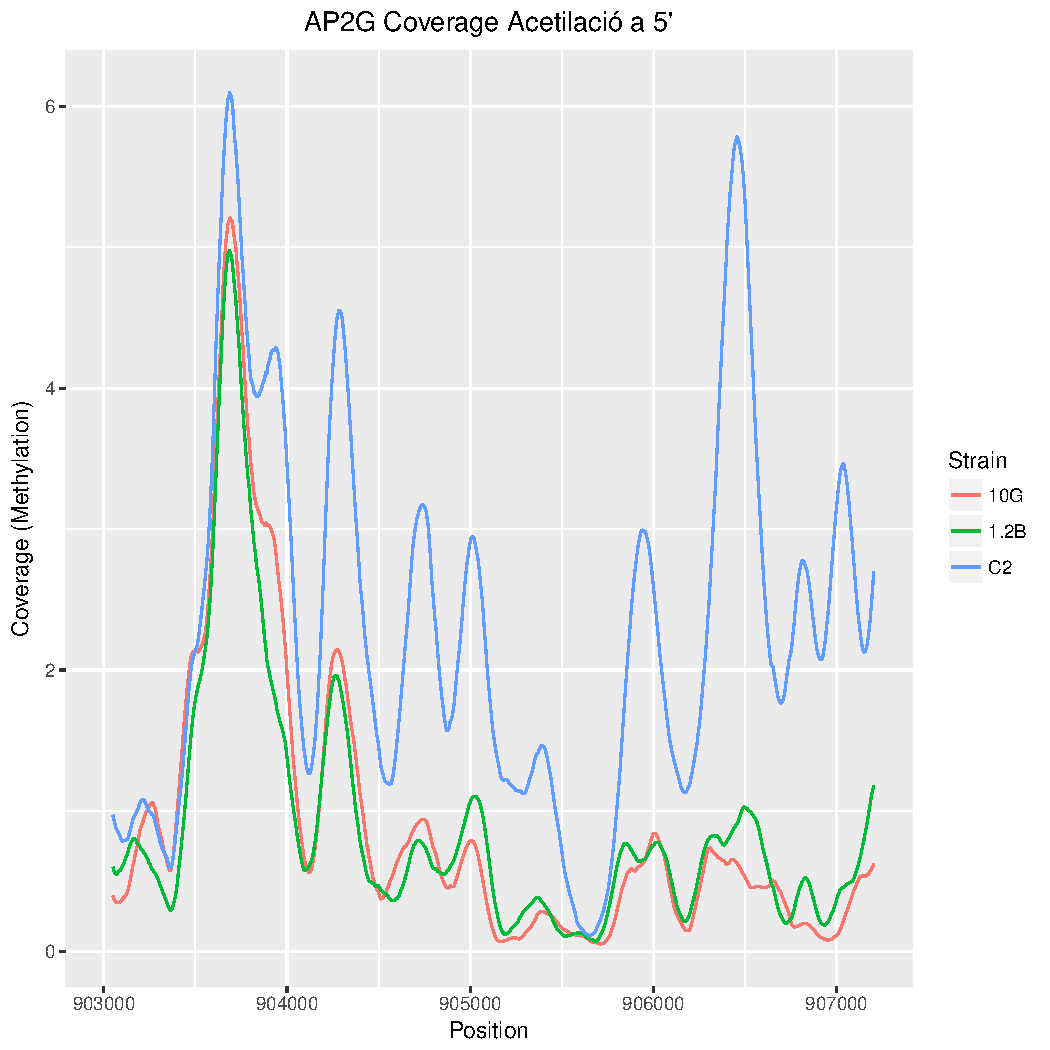
\includegraphics[width=1\linewidth]{figure/plot_ac_5-1} 

\end{knitrout}
\clearpage
\subsection{Acetilació / Metilació (normalitzat per input)}
\begin{knitrout}
\definecolor{shadecolor}{rgb}{0.969, 0.969, 0.969}\color{fgcolor}
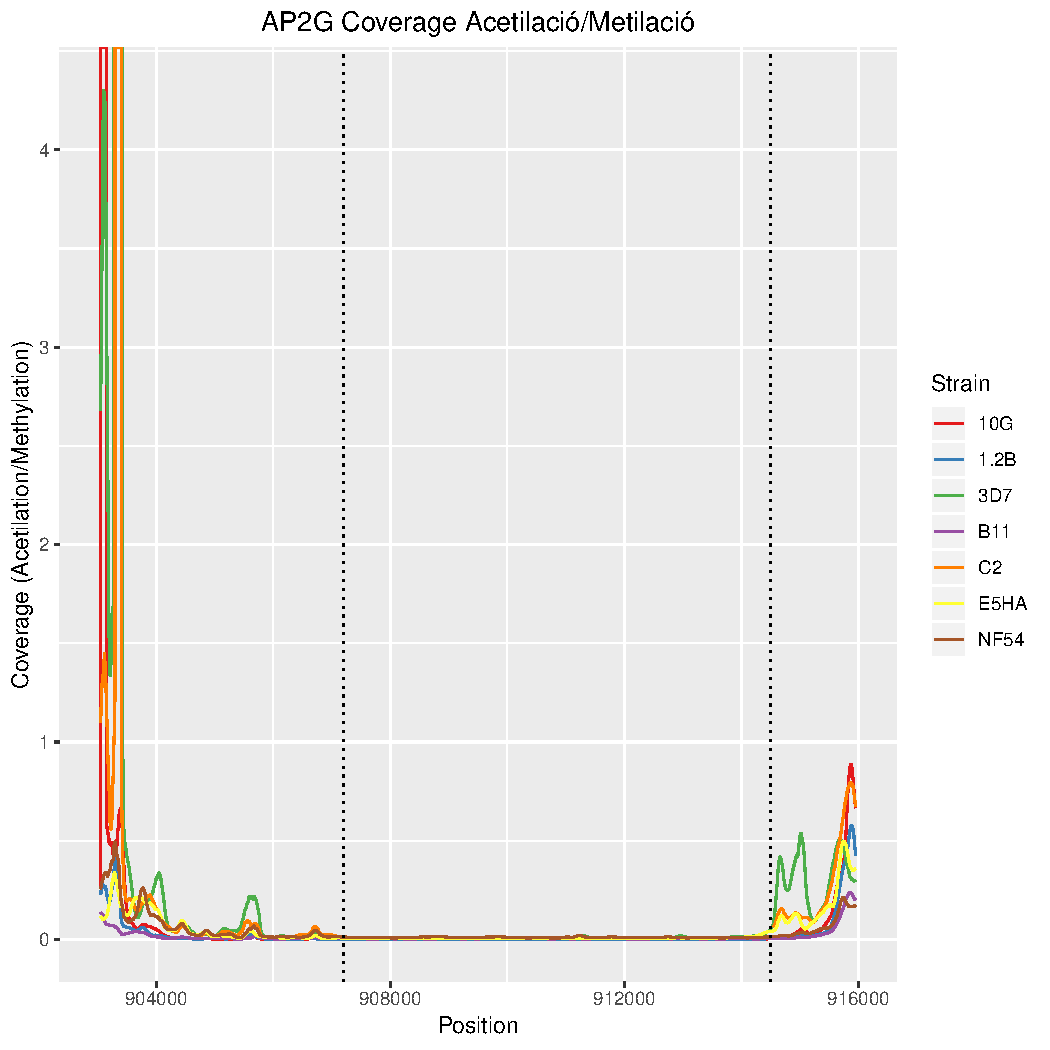
\includegraphics[width=1\linewidth]{figure/Ac_Met-1} 

\end{knitrout}
\clearpage
\subsection{Metilació / Acetilació (normalitzat per input)}
\begin{knitrout}
\definecolor{shadecolor}{rgb}{0.969, 0.969, 0.969}\color{fgcolor}
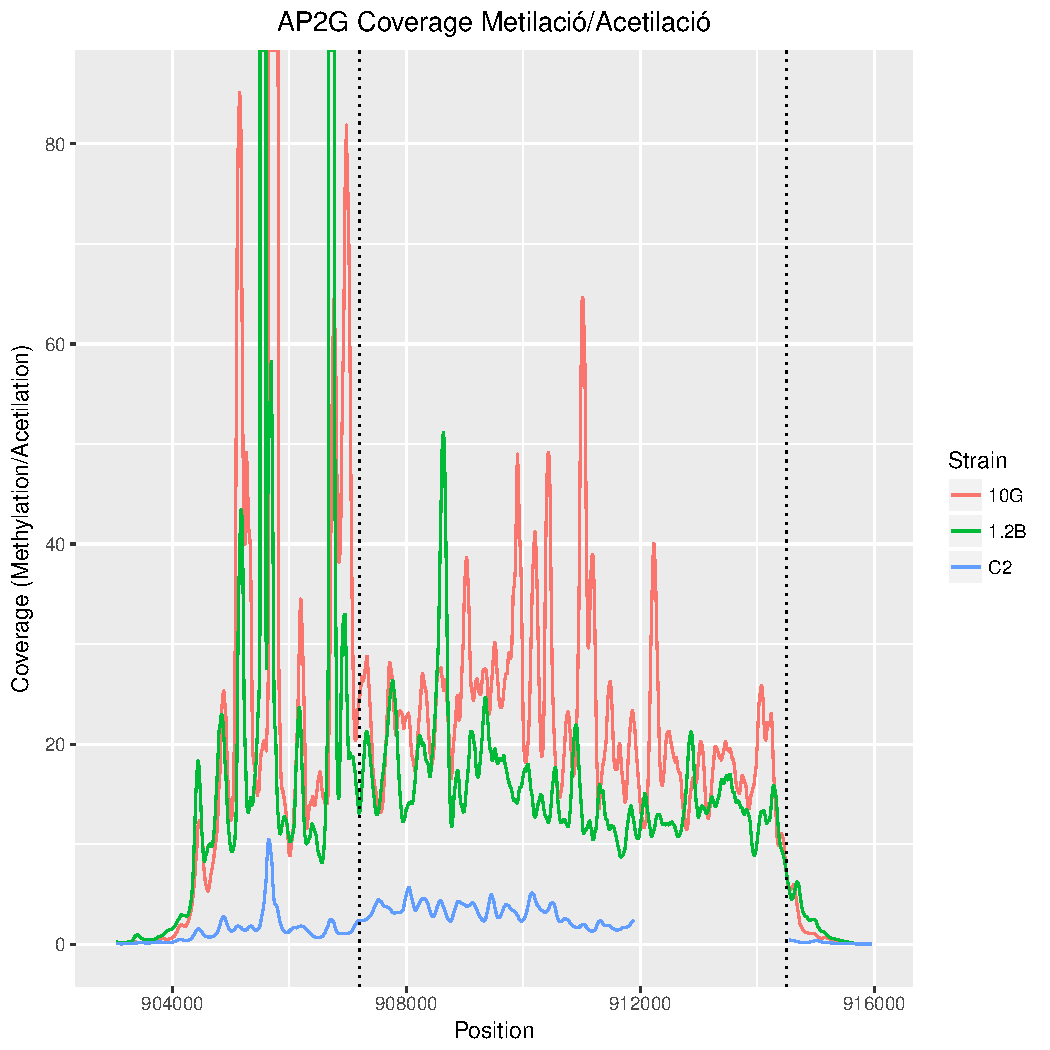
\includegraphics[width=1\linewidth]{figure/Met_Ac-1} 

\end{knitrout}

\end{document}
